
% This LaTeX was auto-generated from MATLAB code.
% To make changes, update the MATLAB code and republish this document.

\documentclass{article}
\usepackage{graphicx}
\usepackage{color}

\sloppy
\definecolor{lightgray}{gray}{0.5}
\setlength{\parindent}{0pt}

\begin{document}

    
    \begin{verbatim}
DoF=[1,5,40];
mu=0;
SigmaSquared=1;
SampleSize=100;

ChiData=zeros(SampleSize,1);
dimDoF=size(DoF,2);
Counter=1;
while Counter<=dimDoF

    %Calculates random varaibles by summing and squaring normal distributed
    %ones
    count=1;
    while count<= SampleSize
        n=DoF(Counter);
        Variables=NormGenerate(n,mu,SigmaSquared);
        ChiData(count,1)=dot(Variables,Variables);
        count=count+1;
    end
    %Plots histogram with distribution imposed
    figure
    histogram(ChiData,'Normalization','pdf')
    hold on
    x=linspace(0,max(ChiData));
    y=pdf(x,DoF(Counter)/2,1/2);
    line(x,y,'LineWidth',2,'Color','g')
    xlim([0,inf])
    ylim([0,1.1])
    legend('Data','Exact p.d.f','Location','northeast')
    xlabel('\chi^{2}_{n} Sample')
    ylabel('Frequency Density')
    print(strcat('Image_11_',num2str(Counter)),'-depsc')
    Counter=Counter+1;
end

function answer = pdf(x,a,b)
    answer=b^(a).*x.^(a-1).*exp(-b.*x)/gamma(a);
end

function Variables = NormGenerate(n,mu,SigmaSquared)
    A=rand((n-mod(n,2))/2+mod(n,2),1);
    B=rand((n-mod(n,2))/2+mod(n,2),1);
    Phi=2*pi*A;
    V=-2*log(1-B);
    X=mu+SigmaSquared*sqrt(V).*cos(Phi);
    Y=mu+SigmaSquared*sqrt(V).*sin(Phi);
    Variables=[X;Y(1:n-(n-mod(n,2))/2-mod(n,2),1)];
end
\end{verbatim}

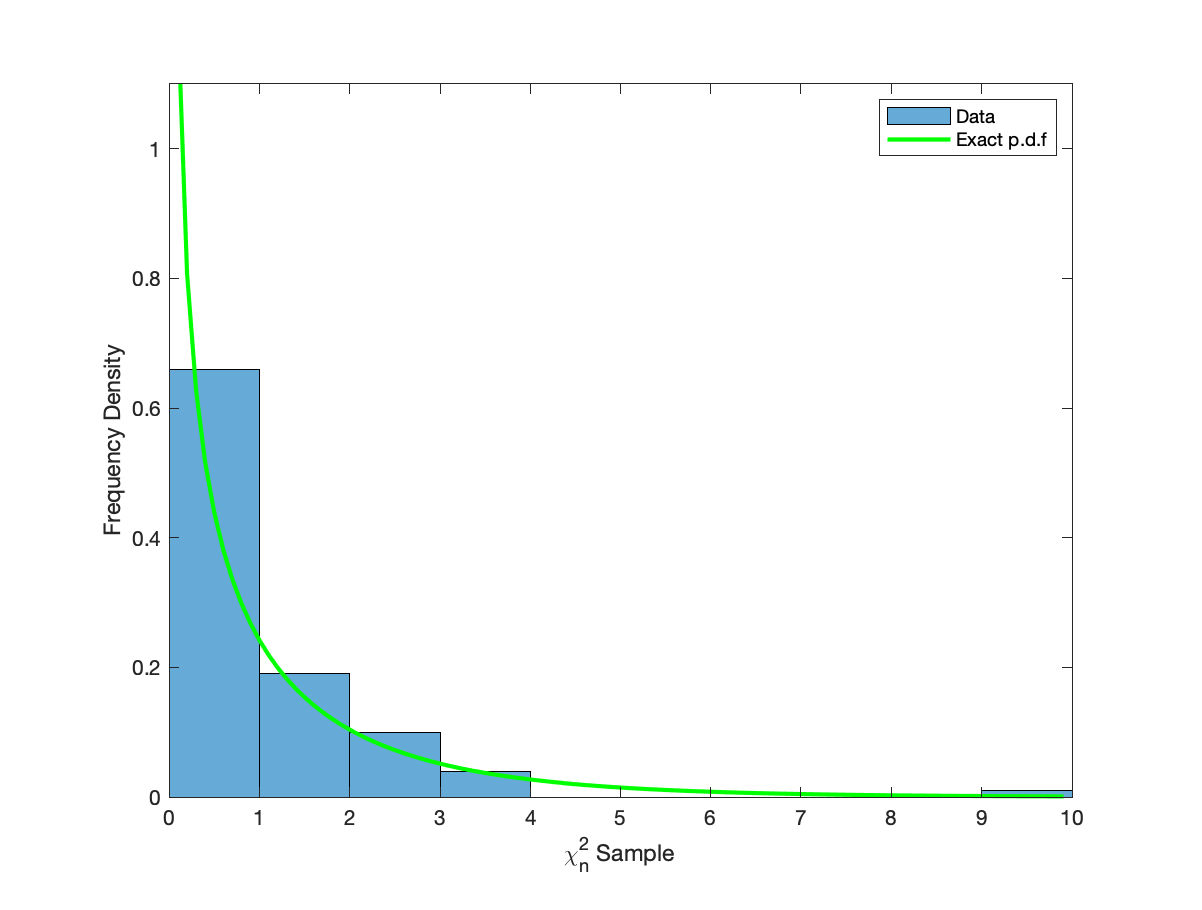
\includegraphics [width=4in]{Code_13_1_01.eps}

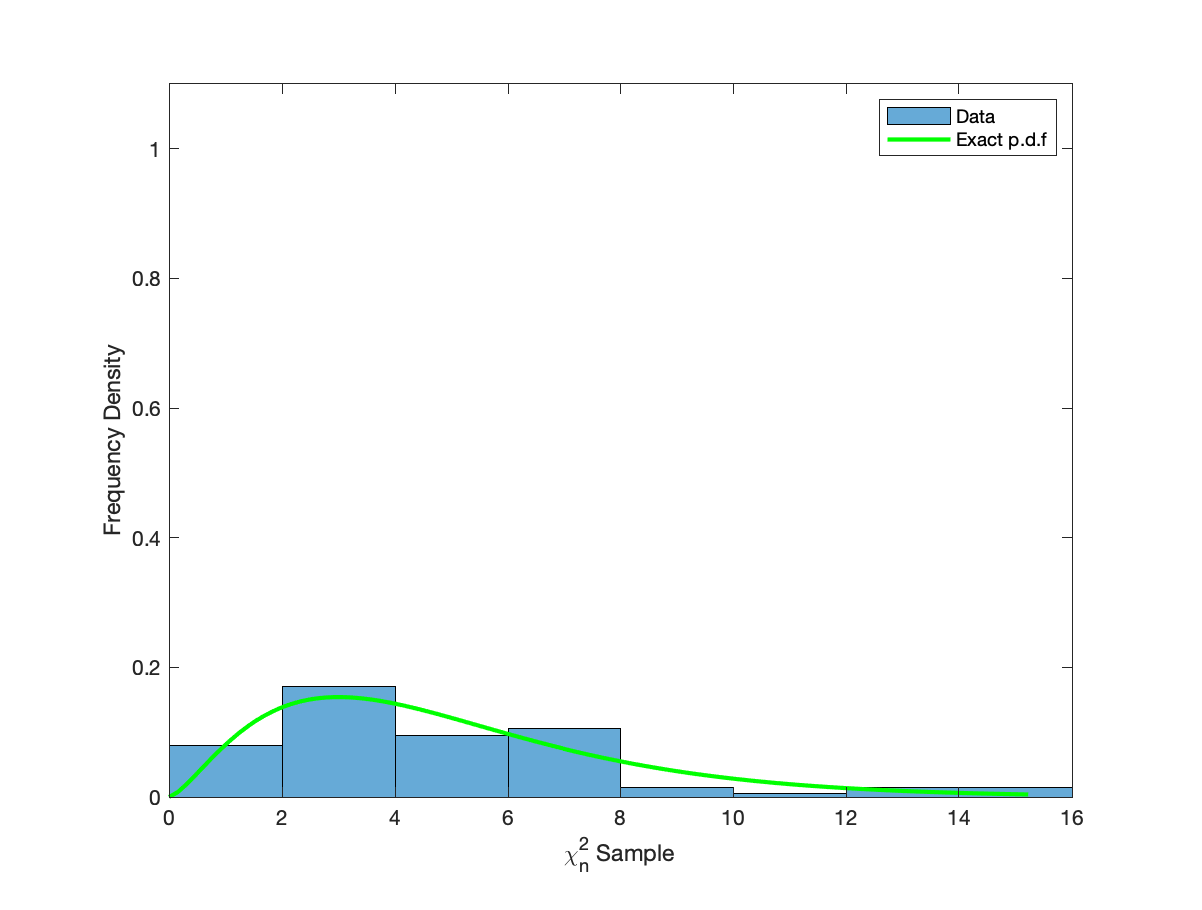
\includegraphics [width=4in]{Code_13_1_02.eps}

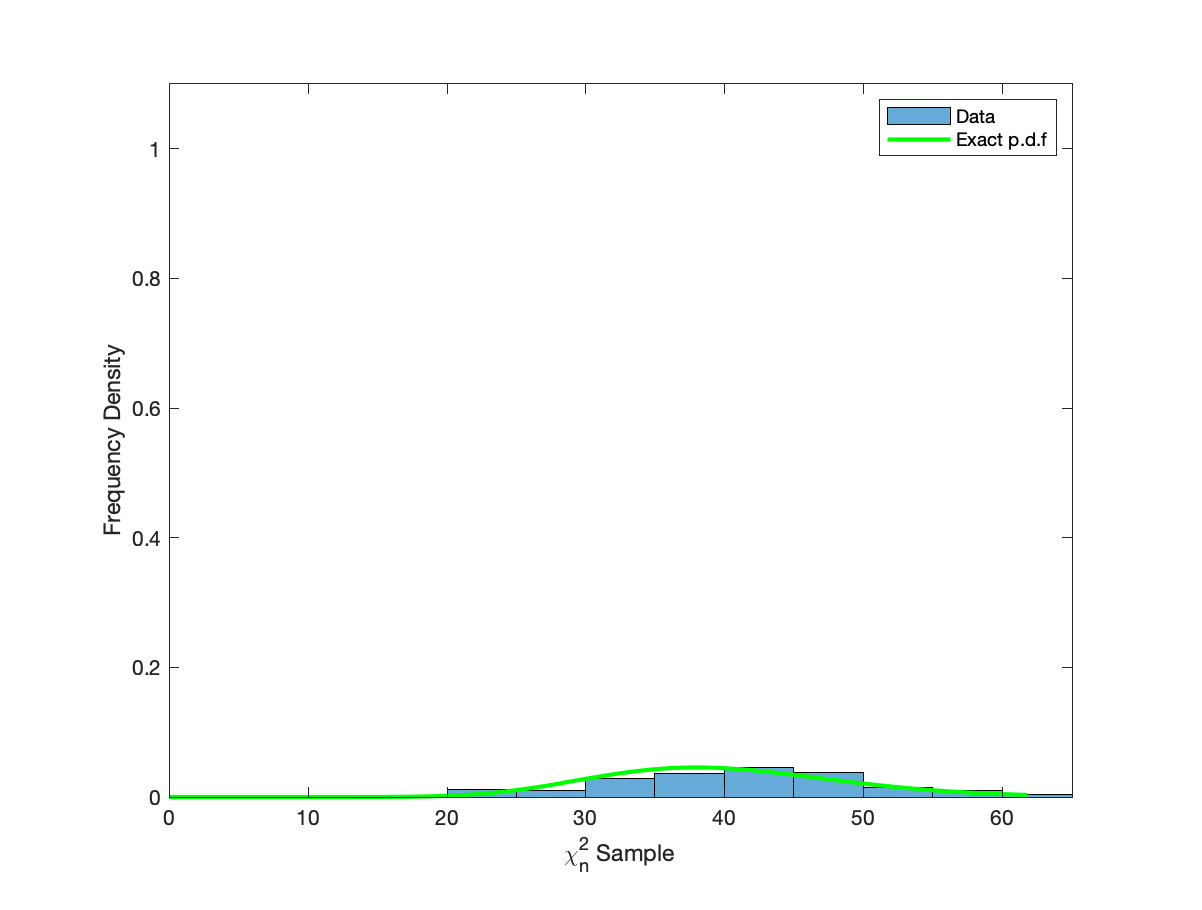
\includegraphics [width=4in]{Code_13_1_03.eps}



\end{document}
    
